\chapter{CMS DETECTOR}
\label{chap:Detector}

The CMS Detector is a multi-purpose detector designed to accurately measure the energy of all particles produced in proton-proton collisions. Figure~\ref{fig:CMS}  shows a schematic of the detector as a whole. Each sub-detector will be described in more detail in the following sections. Moving radially outward from the interaction point, the sub-detectors are the silicon pixel and strip tracker (Section~\ref{sec:Tracker}), the electromagnetic calorimeter (Section~\ref{sec:ECAL}), the hadron calorimeter (Section~\ref{sec:HCAL}), and the muon system (Section~\ref{sec:Muon}). 

\begin{figure}[h!]
	\centering
	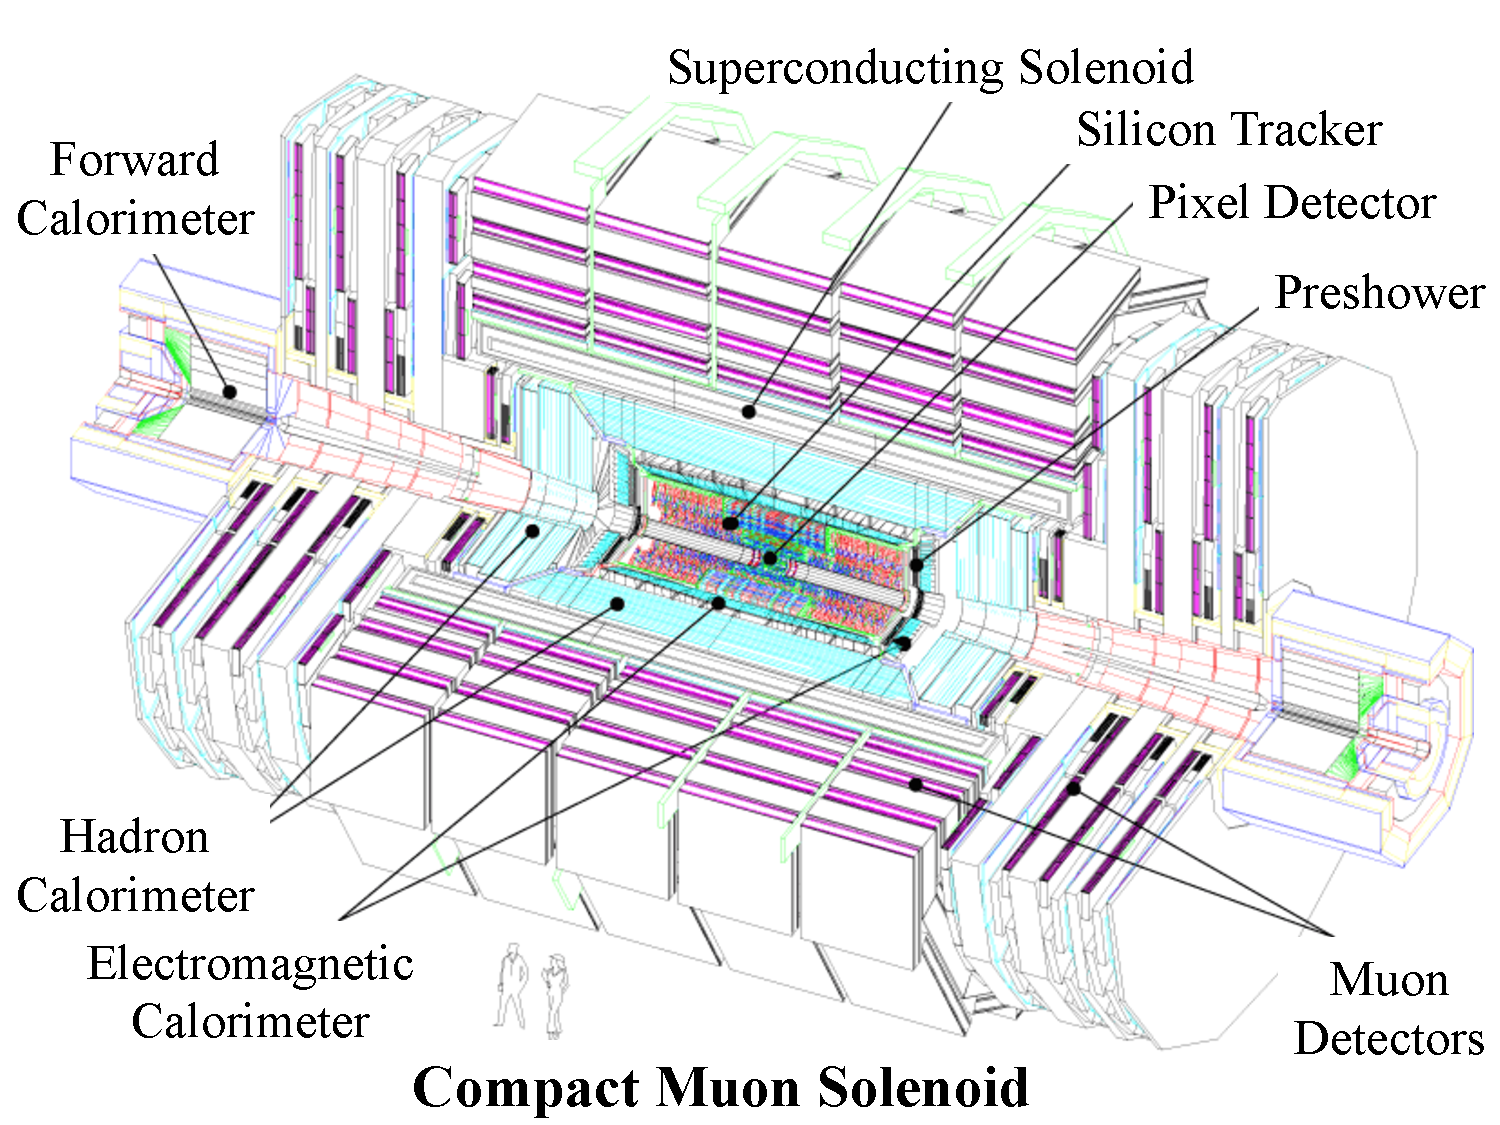
\includegraphics[width=0.45\textwidth]{Figures/Detector/cms_labelled.pdf}
         \caption{Schematic of the CMS detector.
	}
    	\label{fig:CMS}
\end{figure}

\section{Coordinate System}
\label{sec:coordinates}
The origin of the CMS detector coordinate system is located at the nominal collision point. The $z$-axis is oriented along the beam direction, with the positive $z$-axis pointing in the counter-clockwise direction when viewing the LHC from above. The $y$-axis points directly upward, and the $x$-axis points toward the center of the LHC. The $xy$-plane is referred to as the transverse plane.

Due to the nature of particle collisions, however, Cartesian coordinates are often not the most convenient. Because protons are not elementary particles, it is actually the individual quarks or gluons within the proton that interact during the collision. This means that the collision will not be at rest in the lab frame, but will have some non-zero velocity along the $z$-axis. To deal with this it is beneficial to use coordinates that are invariant under boosts in the $z$ direction. CMS follows the particle physics convention of describing the position of a particle in terms of its transverse momentum, azimuthal angle, and pseudorapidity. The transverse momentum \pt is defined as the magnitude of the momentum in the $xy$ plane. The azimuthal angle $\phi$ is defined in the transverse plane, with $\phi  = 0$ corresponding to the positive $x$-axis. Finally, the pseudorapidity is defined as $\eta = -\ln{\tan{ (\theta / 2 )} } $, where the polar angle $\theta$ is measured from the $z$-axis.

\section{Superconducting Solenoid}
\label{sec:magnet}

At the heart of the CMS detector is the superconducting solenoid. The CMS magnet is capable of producing fields up to 3.8 T. 

\section{Tracker}
\label{sec:Tracker}

pixel and strip

\section{Electromagnetic Calorimeter (ECAL)}
\label{sec:ECAL}

Very important. Finds photons.

\section{Hadron Calorimeter (HCAL)}
\label{sec:HCAL}

brass sampling calorimeter

\section{Muon System}
\label{sec:Muon}

The muon sub-system is located outside of the solenoid and is embedded in the return yoke for the magnetic flux. Three different types of detectors are used in the muon system: drift tube chambers (DTC) = positively charged wire within gas volume. Muon knocks electrons off atoms in the gas, which are attracted to the wire. Can determine where electrons hit and where the muon was from the wire to get 2 coordinates for its position. Barrel
Cathode strip chamber (CSC) = better for high flux areas. Crisscrossing positive and negative wires. Muons knock off electrons, which go to positive wires. Ions move toward negative wires. Two position coordinates. Endcaps.


